\documentclass[10pt]{article}
\usepackage[margin=1.8cm]{geometry}
\usepackage{booktabs}
\usepackage{amsmath}
\usepackage{graphicx}
\usepackage[hidelinks]{hyperref}
\setlength{\parskip}{3pt}
\setlength{\parindent}{0pt}

\begin{document}

\begin{center}
{\Large Arm actions at 3.5\,Hz vs 1\,Hz: what the references demand and what the policies do}\\[3pt]
Companion to \texttt{action\_scale.pdf}. pal\_mjlab \texttt{omm/action-scale-graphs}, October 2026.
\end{center}

\textbf{Notation.} Setpoint $q_{sp} = q_0 + \alpha a$ with $\alpha = 0.25\,\tau_{\max}/K_p$ (rad per action
unit). The action-rate penalty is $-0.1\,\lVert a_t - a_{t-1}\rVert^2$, computed on the \emph{raw} policy
output (mjlab's \texttt{action\_rate\_l2}). Penalties are given as a share of the largest per-step
tracking reward (the six tracking weights sum to 5; both are scaled by $\Delta t$).

\textbf{Data.}
\begin{itemize}
  \setlength{\itemsep}{0pt}
  \item Figure~\ref{fig:demand}: the \texttt{dev} references alone (1,294 clips), no policy.
  \item Figure~\ref{fig:policy}: the two D27 A/B checkpoints (PPO-Sim, iteration 999, same seed), played
  the benchmark way on 96 stratified \texttt{dev} clips (first 10\,s, deterministic, no noise; about
  28k steps each).
  \item Only the left arm is shown; the right arm is the mirror. Two leg joints are included for scale.
  \item Scripts: \texttt{scripts/supermimic/action\_stats.py}, \texttt{docs/supermimic/m1/make\_action\_scale\_figures.py}.
\end{itemize}

\begin{figure}[h]
\centering
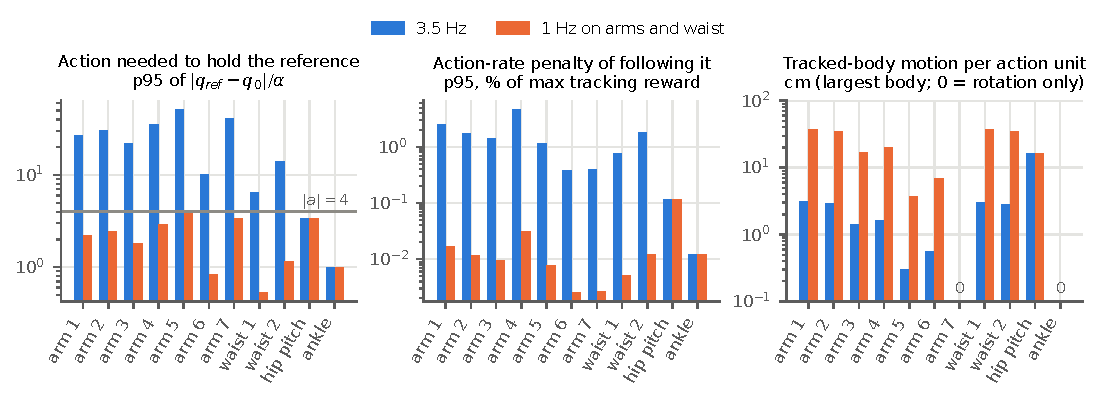
\includegraphics[width=\linewidth]{figures/reference_demand.pdf}
\caption{\textbf{What the references demand, per joint.}
\textit{Left:} action needed to hold the reference pose, $|q_{ref}-q_0|/\alpha$. At 3.5\,Hz every arm joint
needs 10--50 units (p95). \textit{Middle:} action-rate penalty of following the reference. It is the
same for all arm joints, $\approx 0.4$--$5\%$ each at p95. \textit{Right:} how far one action unit
moves the tracked bodies, $\alpha\times$lever arm. Joints 1--4: 1.4--3.1\,cm; joints 5, 6: 0.3,
0.6\,cm; joint 7: 0, because it only rotates the wrist body about its own origin.}
\label{fig:demand}
\end{figure}

\begin{figure}[h]
\centering
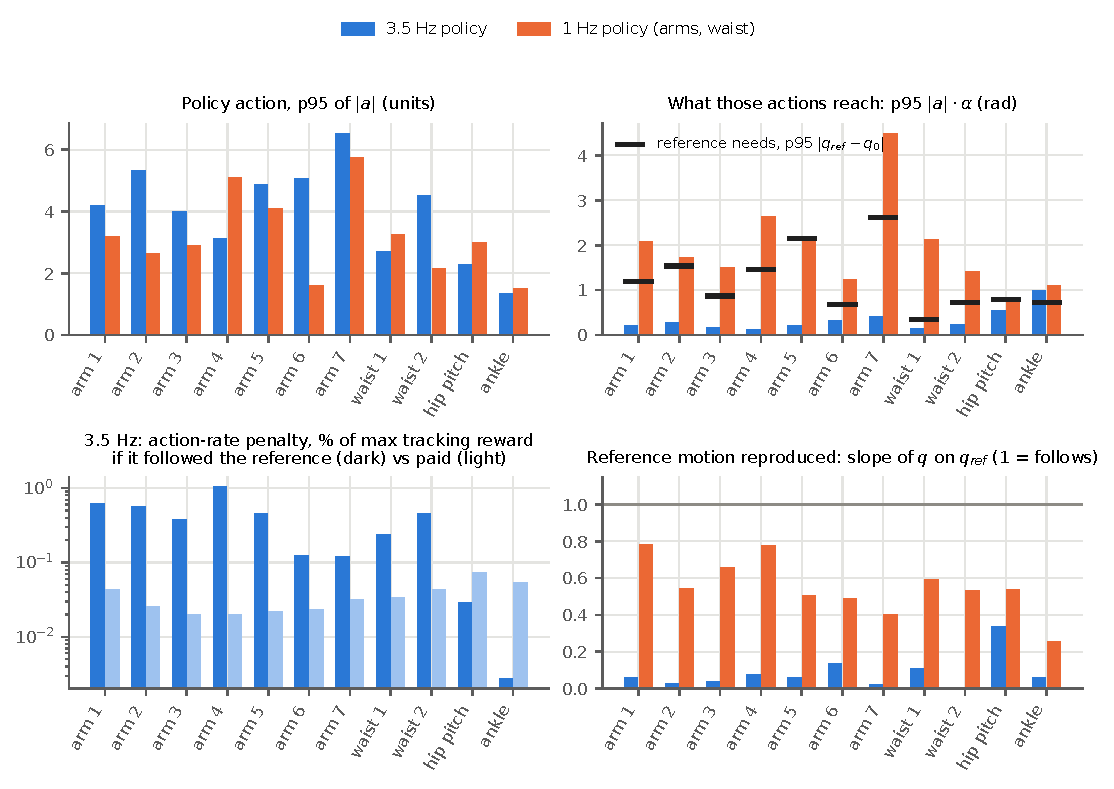
\includegraphics[width=\linewidth]{figures/policy_actions.pdf}
\caption{\textbf{What the trained policies do.}
\textit{Top left:} both policies keep $|a|$ within a few units (p95 3--6.5).
\textit{Top right:} at 3.5\,Hz those units reach only 0.12--0.58\,rad of setpoint, against the 0.68--2.62\,rad
the references need; at 1\,Hz they reach 1.25--4.48\,rad.
\textit{Bottom left:} at 3.5\,Hz, following the references would cost 6.8\% of the maximum tracking
reward per step on average (p95 26\%) for the arms alone. The policy pays 0.37\%.
\textit{Bottom right:} share of each joint's reference motion the policy reproduces. At 3.5\,Hz it is
0.01--0.14 for \emph{every} arm and waist joint; at 1\,Hz it is 0.40--0.78.}
\label{fig:policy}
\end{figure}

\section*{Why the WBC report saw it mainly on joints 5--7}

\begin{enumerate}
  \setlength{\itemsep}{1pt}
  \item \textbf{The action-scale problem is arm-wide.} All seven arm joints have
  $\alpha \approx 0.04$--$0.06$ at 3.5\,Hz. All need 10--50 units to hold their references, and all
  make following them expensive (Figure~\ref{fig:demand}, left and middle). In the SuperMimic task the
  3.5\,Hz policy freezes the \emph{whole} arm and the waist (Figure~\ref{fig:policy}, bottom right).
  \item \textbf{What differs per joint is how much reward one action unit can buy}, i.e.\
  $\alpha \times$ lever arm $\times$ how much the reward weighs that body.
  \begin{itemize}
    \item Joints 1--4 move the tracked elbow and wrist 1.4--3.1\,cm per unit even at 3.5\,Hz.
    \item Joints 5 and 6 move them 0.3--0.6\,cm per unit.
    \item Joint 7 moves them 0\,cm. It only rotates the wrist body, by $\alpha \approx 3.6^\circ$ per
    unit, which is small against the orientation term's $0.4$\,rad ($23^\circ$) scale averaged over the
    tracked bodies.
  \end{itemize}
  \item \textbf{The WBC task concentrates its arm signal on the end effector}: the target position is an
  actor input, and the end-effector body terms are rewarded. So the centimetre-scale effect of joints
  1--4 is enough for PPO to learn them; joints 5--7, with almost no position effect and a flat
  orientation term, stay at $q_0$. SuperMimic tracks 14 bodies averaged together, of which the arm is
  6, under the full action-rate penalty, so even joints 1--4 don't earn enough. This point is an
  interpretation consistent with both studies, not measured in the WBC task.
  \item \textbf{The lever-arm effect stays at 1\,Hz.} $\alpha$ grows $12\times$ on every arm joint, but
  joint 7 still moves no tracked position. Its reproduction (0.40) is the lowest of the arm, and joint
  5's error does not improve (0.89 vs 0.95\,rad mean $|q-q_{ref}|$).
\end{enumerate}

\textbf{Takeaway.} Choose $\alpha$ per joint from the reward the joint can affect, not only from
$\tau_{\max}/K_p$. That is the WBC report's conclusion, and here it applies to the whole arm, with the
wrist as the extreme case.

\end{document}
